\chapter{Introduction} \label{chapter-introduction}

% \vspace*{\fill}
% \epigraph{DISTRIBUTION QUOTE?}{}
\epigraph{Cities are the crucible of civilization, the hubs of innovation, the engines of wealth creation and centers of power, the magnets that attract creative individuals, and the stimulant for ideas, growth, and innovation.}{Geoffrey West}
% \cite{westScaleUniversalLaws2017}
%``cities..% the 'force' we need to postulate account for the central role of cities in economic life is of exactly the same character as the 'external human capital'}{Robert E. Lucas Jr., \textit{ON THE MECHANICS OF ECONOMIC DEVELOPMENT (1988)}}

%The question of how wealth is created and distributed has been central to Economics since the discipline emerged. ** ^E ADD GENERAL STATEMENT ABOUT THIS OR MAYBE CUT THIS SENTENCE
% Prior to the industrial revolution, most people live on and worked on the land, primarily producing food, but ownership of the land was highly concentrated. Ownership or lack of ownership  of land was the primary social distinction. Landowners, by definition, controlled access to the means of production and charged for access. The income  they extracted was what economists call economic rent, or more familiarly, land rent.

% Property ownership has been a central form of wealth throughout history. % one of central forms of  wealth and means of building wealth 
% As the primary producer of food
% As the primary source of food, power comes from food, which was the main product. 
%  ADD EXPLANATION % Land ownership traditionally defined the ruling classes. The king would give land as reward. Land is what you would fight wars for. The agricultural surplus , the surplus from the land what allowed civilization and cities to form. Before the industrial revolution, the surplus of  agricultural land. taking ownership used to consolidate wealth and power, in feudalism ownership of land set apart ruling classes/aristocracy, . As pearl buck said "land is everything.." or quote that "the only way to create intergenerational wealth is the rare company that or property ownership.  GIVE EXPLANATION HISTORY OR SUMMARY
% More recently the expansion of European economies across the globe brought huge amounts of land into play and combined with rapidly falling transportation costs, led to a society, especially in the labour-scarce settler societies of North America and Australia with  widely distributed property and  home ownership. 


 Since the industrial revolution, widely distributed property ownership, particularly in North America,  has contributed to the wide and relatively equal distribution of wealth \footnote{The role of housing in wealth accumulation is well known After a detailed  examination of data from the US  Survey of Consumer Finance (SCF) and the Panel Study of Income Dynamics (PSID), Herbert et al. concluded that ``there continues to be strong support for the association between owning a home and accumulating wealth.'' even for among minorities and lower-income households, and that in contrast, renters generally do not see any gains in wealth. \cite{herbertHomeownershipStillEffective2013}} \cite{pikettyCapitalTwentyfirstCentury2014, harrisGrowthHomeOwnership1977, chevanGrowthHomeOwnership1989, andrewsEvolutionHomeownershipRates2011}. % It is a key differentiator between who has built wealth and who hasn't. % ADD FACTS. %This is seen in the racial wealth gap, the immigrant wealth gap, and the youth wealth gap. 
However, property ownership is now going through a great transformation in structure, with financial capital coming to own a larger share of the urban land and housing stock.\cite{farhaReportFinancializationHousing2017, palleyFinancializationWhatIt2007}. For the first time in Canadian history the rate of homeownership has declined, falling from -- in xx to xx in xx \cite{GET_homeownership_rates}. %This is a general shift away from --- to ---- %, is held by financial capital. 
% ^E MORE DETAIL ABOUT THIS %Through changing legal structures, development of financial tools, and ... and 
%increase of property speculators. The result is that the ownership is shifting/ For example, 
In Waterloo 77\% of new housing units are  owned by investors not residents \cite{GET77percent}. %(Change from dATE). Fewer people are able to buy houses and those renting face higher rents and decreased ability to build wealth. 
This process has been called financialization \cite{farhaReportFinancializationHousing2017, hansenFinanceCapitalismFinancialization2014}. 

There is an emerging understanding that this general transformation,  called financialization, affects the accessibility, security, and affordability of housing. 
Because of the significance of housing ownership to wealth distribution, the  financialization of ownership % this shift %/this financiazation
has a growing effect on the overall distribution of wealth.
\cite{tomaskovic-deveyFinancializationCausesInequality2013, palleyFinancializationWhatIt2007, seccarecciaUnderstandingFinancializationHistory2013, nemtinFinancializationHousingSocial2021}. %This is accept SEEN IN XY say.  % \cite{nemtinFinancializationHousingSocial2021}, \cite{}
% DO WE WANT TO SAY THESE ARE THE REFERENCES FOR ESTABLISHING THE EFFECT ON THE OVERALL DISTRIBUTION OF WEALTH- THAT IS ONE OF THE THINGS WE'RE LOOKING AT..

Financialization is being described  %talked about in this way. People working in housing have noted people can be priced out of the city as speculative approaches to housing lead to attempts to claim more rent. This idea has been introduced 
as a contributor to the current housing crisis. What has not explored as much is the systemic effects of financialization. 
% Financialization is key to that idea in understanding what is happening. DEFIE
% The idea of financialization of the housing market has been gaining currency. ^E IN WHAT SENSE? %SAY WHAT IT IS GAINING CURRENCY FOR... AMOUNG WHAT GROUP TO EXPLAIN WHAT... THE HOUSING CRISIS? THEN EXPLIAN BUT IT'S HAS DEEPER/MORE SIGNIFICANT EFFECTS ON SYSTEMS....
 
 
 This thesis is a study of financialization in the context of housing markets. Specifically we explore the systemic effects of the shifting ownership of cities on the capacities of cities to grow. We explore how the effects of financialization go beyond direct effects on distribution of property ownership and access to city space to explore its effects on the ability of cities to thrive and produce wealth. Cities are dynamic wealth-producing centres and land ownership patterns matter to ???. 
 We have built a model  on a model that brings together ....  to explore how .... , we argue that financialization .... and that it may also have dramatic effects on the productivity of cities.

\section{The financialization of housing markets}
 % in particular it's efect on productivity.
Financialization of the housing market refers to the growth in the share of the housing stock controlled by financial institutions and investors and the overall effect this has on the outcomes of the system \cite{farhaReportFinancializationHousing2017, hansenFinanceCapitalismFinancialization2014}. 
This thesis focuses on the potential macro effects of financial capital capturing spatial urban rents. 

 %also a spatial  phenomenon. 
% ^E MAYBE MOVE THIS UP... IT MIGHT BE HELPFUL CONTEXT FOR WHAT YOU ACTUALLY DO, IT BEGINS TO ESTABLISH THE PROBLEM
 % These macro effects are our main interest. % While the term financialization can be used in a variety of ways,
 % are the specific concern of this thesis.  
% These aspects of finacialization have been neglected in the literature.%in the urban system 

There's now a compelling understanding of the value that's created by cities, both empirically and theoretically \cite{jacobsEconomyCities1969, spenceUrbanizationGrowth2009, bettencourtIntroductionUrbanScience2021}, but there's no formal apparatus in standard economic theory for analyzing the distribution of the enormous value created. % that's being created. 
Standard models of the financial operations are spaceless.\footnote{In describing any theory we need to identify the kinds of objects that are theorized. Financial analysis theorizes  assets, debts, flows of revenue and costs, and the rates of change or exchange of these quantities over time. These are inherently spaceless because they are accounting entities, completely independent of location. It matters where a worker or a farm is. It does not matter where and dollar or a rouble is.} 
% since financial analysis theorizes objects such as assets, debts, revenue and cost flows, and the changes in and exchange values of their values over time. These are inherently spaceless because they are accounting entities, independent of location. It matters where a worker or a farm is. It does not matter where and dollar or a rouble is.
Our solution is to explicitly embed the normally spaceless analysis of investment decisions in a spatial model with locational rents. % to spatial rents in an urban system. % to refomulate the 

Our focus is on who captures these rents and how that affects the city. The distribution of locational rents, we believe, goes some distance to explaining core social issues like class structure, inequality, political political power. 
The ultimate goal of this work is to develop a modern urban theory of rent, linking spatial rent, housing markets, and urban production. The following sections introduce how this work fits in the literature and the basic structure the core model, then list the main contribution, and give an outline for the document. 

\begin{figure}[!ht]
    \centering
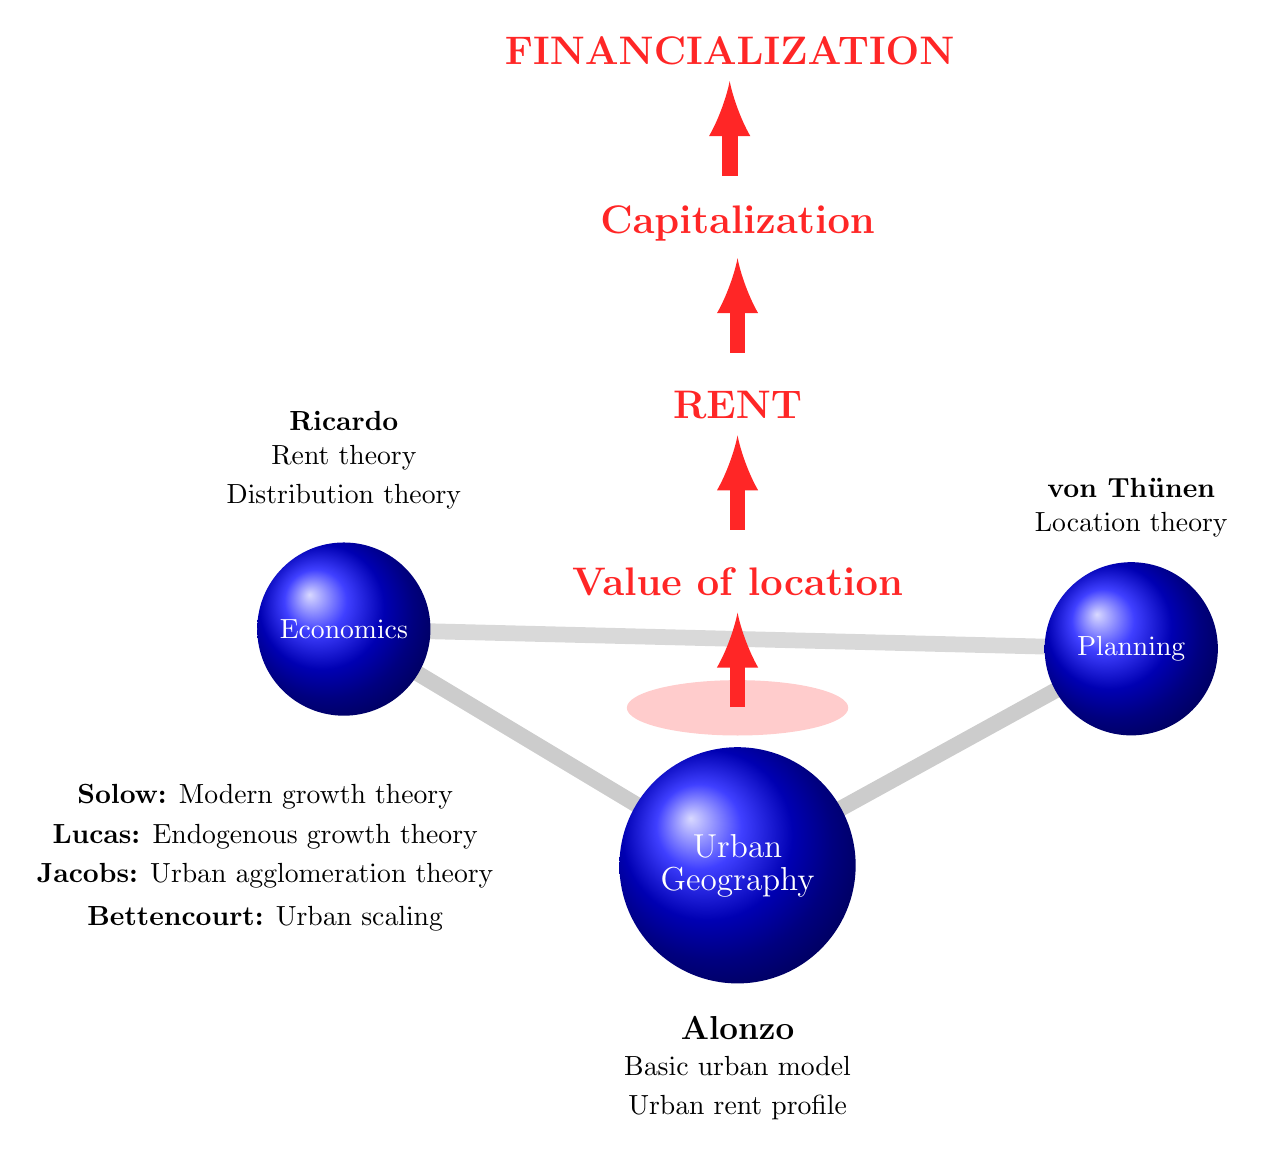
\begin{tikzpicture}{scale=.5}
% find color cotrol for ball. Tind way to stop line short of node
\coordinate (planning) at (5,.75);%PREFACE
\coordinate (economics) at (-5,1);%
    \coordinate (Ricardo) at (-5,1.4);
    \coordinate (Solow) at (-6,1.25);
 \coordinate (geography) at (0,-2); %history
\coordinate (finance) at (0,5); %

\draw [line width=2mm, black!15, ] (planning)--(economics);
\draw [line width=2mm, black!20, ] (geography)--(economics);
\draw [line width=2mm, black!20, ] (geography)--(planning);

%\draw [line width=2mm, black!25, ] (geography)--(finance);
%\draw [line width=2mm, black!20, ] (planning)--(finance);
%\draw [line width=2mm, black!20, ] (finance)--(economics);
%color=black!60!red

 %  \shade [ball color=blue!70] (5,5) circle (1.1cm)node[white] {\textbf{Planning}};
\node [circle,shading=ball,  minimum width=2.2cm, white, align=center] (ball) at (planning) {Planning};
\node [circle, shading=ball, minimum width=2.2cm, white, align=center] (ball) at (economics) {Economics};
\node [circle,shading=ball, minimum width=3cm, white, align=center] (ball) at (geography)[text width=2cm] {\large Urban\\ Geography};

%\node [circle, shading=ball, minimum width=2.4cm, white, align=center] (ball) at (finance)[text width=2cm] {Finance};

%\node at (-.3,-.1) [red] {\Large \textbf{RENT}};

% new stuff
\node at (planning) [above=1.8cm] {\textbf{von Th\"unen}};
\node at (planning) [above=1.3cm] {Location theory};

\node at (Ricardo) [above=2cm, ] {\textbf{Ricardo}};
\node at (Ricardo) [above=1.5cm] {Rent theory};
\node at (Ricardo) [above=1.0cm] {Distribution theory};

% \node at (Solow) [below=1.6cm, align=left] {\textbf{Solow:}};
\node at (Solow) [below=2.1cm, align=left] {\textbf{Solow:} Modern growth theory};
\node at (Solow) [below=2.6cm, align=left] {\textbf{Lucas:} Endogenous growth theory};
\node at (Solow) [below=3.1cm, align=left] {\textbf{Jacobs:} Urban agglomeration theory};
\node at (Solow) [below=3.65cm, align=left] {\textbf{Bettencourt:} Urban scaling};

\node at (geography) [below=1.8cm] {\textbf{\large Alonzo}};
\node at (geography) [below=2.3cm] {Basic urban model};
\node at (geography) [below=2.8cm] {Urban rent profile};

%\node [circle, shading=ball, minimum width=2.4cm, white, align=center] (ball) at (finance)[text width=2cm] {Finance};
\fill[red!20] (0,0) ellipse (40pt and 10pt);
%\node[red]at (1.2,0) {\large SPACE};

\begin{scope}[shift={(0,-.34)}]
\draw [line width=2mm, red!85, -latex ] (-.1, 7.1)--++(0,1.2)node[above=-.1] {\Large \textbf{FINANCIALIZATION}};
\draw [line width=2mm, red!85, -latex ] (0, 4.85)--++(0,1.2)node[above=-.1] {\Large \textbf{Capitalization}};
\draw [line width=2mm, red!85, -latex ] (0, 2.6)--++(0,1.2)node[above=-.1] {\Large \textbf{RENT}};
\draw [line width=2mm, red!85, -latex ] (0, .35)--++(0,1.2)node[above] {\Large \textbf{Value of location}};
%\draw [line width=2mm, red!85, -latex ] (0, -2)--++(0,-.8)node[above=-.1]  {\Large \textbf{SPACE}};
\end{scope}

\end{tikzpicture}

\caption[Linking space and urban rents to the effects of financialization.]{Space and urban rents play a foundational role in urban economics, geography, and planning. We extend the the analysis of urban rents to model the effects of financialization.}
\label{fig-fields}
\end{figure}

\section{Position in the literature}
This work draws together insights from urban economics, geography, and planning. The central, shared concern all three fields is geographic space. Locational value explains the dynamics of economic development, the spatial distribution of human activities, and urban form.  

In all three disciplines, locational value gives rise to land rents, which is for us the link to distribution, financialization, and continuing productivity.  
Figure~\ref{fig-fields} illustrated both the synthetic aspect of our analysis and the direction in which we develop existing work. % The organizing principle in the spatial models of all three disciplines is an economic variable, land rent, % The three disciplines share a simple economic insight.

Classical economist David Ricardo \cite{ricardoEssayInfluenceLow1815} elaborated the theory of land rents in 1815. Johann von Th\"unen \cite{vonthunenIsolirteStaatBeziehung1826} %(1783 -- 1850) 
produced the first serious treatment of spatial economics and economic geography, apparently independently in 1826. In 1961 William Alonzo (and others) \cite{alonsoModelUrbanLand1960} applied the  Ricardian and von Th\"unen theory to the urban system, launching modern urban theory. Meanwhile in economics, Solow \cite{solowContributionTheoryEconomic1956} set off a flood of work on  economic growth growth that  spilled into urban theory through through Jacobs \cite{jacobsEconomyCities1969}, Lucas \cite{lucasMechanicsEconomicDevelopment1988} and Bettencourt et al.\cite{bettencourtGrowthInnovationScaling2007}. 

% 3rd spaceless finance..
% We begin in the region of overlap among the three disciplines with the fundamental linking construct, space. 
All three fields have central theories built around %build their theories around  
the value of location, which is essentially the % we emphasize is expressed as 
locational rents, a concept well developed by classical economists like David Ricardo. Our contribution is to extend the the analysis of urban rents to take into account the effects of financialization.


\section{Modelling the financialization of an urban housing market}
% We take a step beyond integrating labour markets in a city, to studying the distributional effects: who gets the surplus, what does that mean for the class structure, and ultimately the productivity of cities. 
In order to develop an analysis of the distributional effects we have to build a model with three components: a housing market that distributes income and housing, a financialization process, and a production system. 
% The first component, the market model, is illustrated in 
% Figure~\ref{Figure-impacts} shows the main effects  that  arise from the growing financial sector participation in the housing market. 

Figure \ref{Figure-impacts} shows the first component, the market model.
It shows two primary effects financialization has on the housing market: how it allocates % The housing market allocates both 
the housing stock, and how it allocates the \glspl{rent} generated by the urban system. % as illustrated in Figure \ref{Figure-impacts}. PHRASE SO IT'S CLEAR THESE ARE EFFECTS 
% In the analysis developed in this thesis, % Our argument is that
The first effect of financialization, on housing allocation, arises because tenants replace owners. While owner-occupiers share in the growing land rents generated by urban agglomeration effects, tenants do not. As a result, a declining fraction of urban residents accumulate capital through their participation in the housing market, and therefore fewer enter the class of workers with both wage and capital income defined by John Roemer \cite{roemerGeneralTheoryExploitation1982}. 

\begin{figure}[!ht]
    \centering
    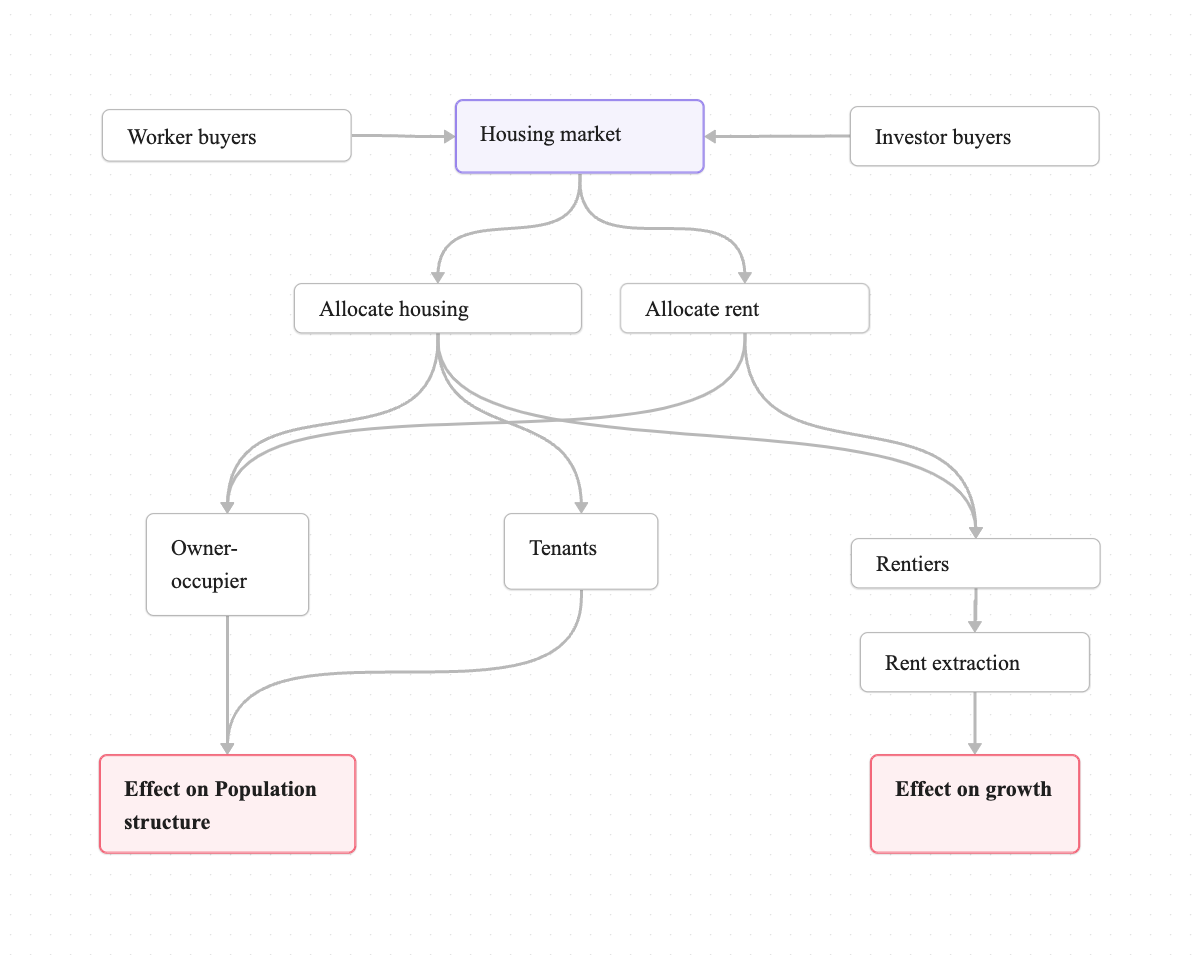
\includegraphics[scale=.60]{fig/flow_impacts.png}
    \label{Figure-impacts}
\caption[The housing market component of the model.]{The housing market component. Financialization affects both  the allocation of housing and its allocation of rents.}
\end{figure}


\begin{figure}[!ht]
    \centering
    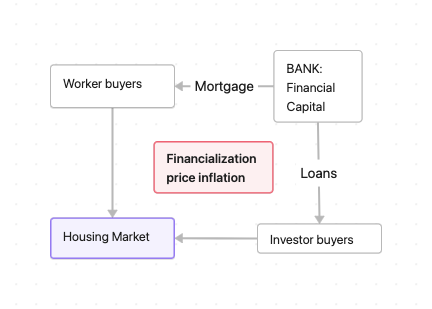
\includegraphics[scale=.70]{fig/flow_financialization.png}
    \label{fig-financial-cycle}
    \caption[The financialization component of the model.]{The financialization component. There is a feedback loop in which new investors drive up demand and thus drive up prices.}
\end{figure}

The second effect of financialization on the market is in the allocation of rents. Rents generated by the agglomeration economies in the urban system are diverted to largely non-resident owners, away from investment in local production or amenities, as tenants replace owner-occupiers. % are gradually replaced by tenants. 


Figure \ref{fig-financial-cycle} illustrates the second component of our model, the financialization process. We develop an explicit model of investor behaviour to explain the market decisions of buyers and the role of financial capital. 
The key observation is that investors enter the housing market. In doing so they drive up prices by increasing total demand. The rising price generates an expectation of capital gains, which enter the investors' calculations. Investors have, as research shows, better access to capital than most new entrants to the housing market. When the financial sector, represented by the bank, the figure, % in Figure\ref{fig-financial-cycle}, 
makes more capital available, the pattern of ownership shifts, as illustrated above. % The theory of financialization is discussed in detail in Chapter ~\ref{chapter-financialization}.

\begin{figure}[!ht]
    \centering
    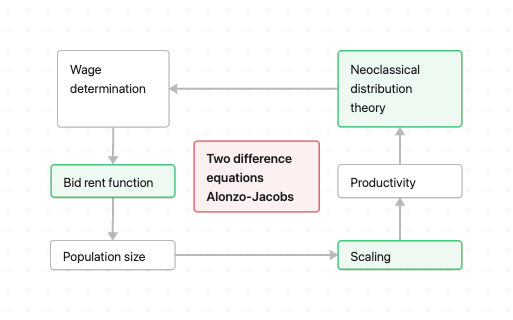
\includegraphics[scale=.7]{fig/flow_Alonzo-Jacobs_cycle.png}
    \label{fig-Alonzo-Jacobs-cycle}
\caption[Production system.]{The production system component, incorporating the urban scaling of wealth in the urban spatial model. We name this coupling of two difference equations the Alonzo-Jacobs cycle.}
\end{figure}

Figure \ref{fig-Alonzo-Jacobs-cycle} illustrates the third component, the model of productivity incorporating agglomeration effects. %the productivity of cities, incorporates the productivity of cities.  
A fundamental feature in recent empirical work on scaling laws is % demonstrated in the recent literature on scaling laws: 
the persistent relationship between population and productivity. The productivity of cities increases superlinearly with population. Cities are the locus of a positive feedback loop with rising populations raising productivity, and rising productivity attracting more people and resources, a theoretical argument associated with the work of Jane Jacobs \cite{jacobsEconomyCities1969}, with strong empirical support from recent work on the scaling of urban productivity  \cite{bettencourtGrowthInnovationScaling2007, bettencourtOriginsScalingCities2013, dongUnderstandingMesoscopicScaling2020, loboUrbanScalingProduction2013}.

Our model brings together an urban spatial model with a model of the scaling of wealth in urban centers. %, using an approach similar to that developed in modern growth theory.
% that we discuss in Chapter ~\ref{chapter-rent}. 
% In that chapter we ground the observation in  \gls{neoclassical growth theory} and recent empirical and theoretical work on \gls{urban scaling}. 
We incorporate that scaling result into the standard urban model, building of the work of William Alonzo and others. %associated with 
We call the combined model the\cite{alonzoTheoryUrbanLand1960}, calling the combined sub-model the 
\gls{Alonzo-Jacobs cycle} because there is a positive feedback between population size and wages. This feedback loop will be vulnerable if financialization extracts the new wealth generated by agglomeration effects, reducing wage growth and therefore the ability of the city to grow, because wage growth is what drives population growth and further agglomeration.
% We describe The Alonzo model in Chapter ~\ref{chapter-space}.
The green boxes in the figure represent the theoretical justification of the primary simplifications in the model. 
% We call the combined sub-model the \gls{Alonzo-Jacobs model}, then combine that with an approach to the scaling of wealth based on the growth and agglomeration work in Chapter \ref{chapter-growth}, on growth.

% When these components are  combined,  
Combining these three components, we have an extended theory of urban rent built on a foundation of theory that goes back to the \gls{classical economics} around the beginning of the 19$^{th}$ century and incorporating modern growth theory and modern urban theory. 

The resulting model suggests two basic hypotheses:
\begin{enumerate}
    \item Financialization of the housing market will result in the tenantization of the urban middle class as financial capital acquires more of the housing stock. % vs decline of the urban middle class
    \item Financialization of the housing market will result in reduced growth of urban productivity as the flow of rents is diverted from real investment to the financial sector.
\end{enumerate} 

\section{Contributions}

The overall goal is to provide a theory of the relationship between financialization and urban productivity. The main contributions towards achieving this goal are:
\begin{enumerate}
    \item  Incorporating \gls{classical rent theory} into an \gls{agent-based} urban model. This requires modelling how \gls{Ricardian rent theory}, a theory of distribution based on an agricultural economy, applies % provides the transmission mechanism
in an economy driven by human capital \gls{agglomeration} effects within the urban system. 

    \item Allowing the creation and distribution of rents to influence urban growth, productivity and  population structure. This requires articulating the links between the wealth production of cities and how the urban system evolves.

    \item Incorporating current research on \gls{urban scaling} into the core spatial urban model.  This requires drawing on empirical work to formalise the scaling relationship, which embeds productivity in an urban model. % we argue is an elegant way to model a an urban system with production. % We show how understanding how complex systems scale provides an 

    \item Constructing an urban \gls{agent-based model} that is consistent with {neoclassical growth theory}. We show how the neoclassical framework can be implemented in the agent-based framework, and make a case for the usefulness of the approach in linking urban rents and productivity. %Chapter \ref{chapter-methodology} discuses methodological implications of this approach.

    \item Integrating \gls{financial capital} into a standard spatial model of the urban system, making an explicitly spatial model of the financial structures, which have traditionally been formalized in a spaceless way.
% We are not aware of any urban simulation models that
% We introduce capital within this framework in a novel way. %as we do to examine the outcomes that concern us.
    
    \item Integrating financial capital into an \gls{overlapping generations} population model of the urban system and %While financial assets are central to most overlapping generations models, we %. Our innovation is to 
articulating the movement of financial capital though the urban land market. 
% SOMETHING LIKE Adding space to finance which has been spaceless.
    
    \item Using an agent-based model to examine how financial markets impact urban \glspl{land market},
% We began with the fact that there is growing policy concern about the financialization of  housing. We have produced 
producing a formal simulation model that illustrates the process of housing financialization. 

    \item Testing for \gls{hysteresis} resulting from the business cycle in the urban system and exploring the \gls{resilience} implication's of the core spatial economic model.
% There are two types of resilience questions when any system is shocked, does it return to an equilibrium state, the stability question, and does it return to the same kind of equilibrium -- the hysteresis question. % We focus on the latter question.  

    \item Building a model that is easily extended to explore a range of issues, and used to evaluate policy options. 
The model combines clear and explicit theoretical assumptions with careful and transparent implementation of the logic. % in code.. %flexible Python code.
    % \item Providing a model that we believe
We have taken care to allow for  both theoretical and policy-relevant extensions in the simulation,  building a base model that aims to be as simple as something like Alonzo's urban model \cite{alonsoLocationLandUse1964}, but 
% To be useful in policy discussions, a model must  
simulates the relevant system features and can incorporate a range of intervention types. %way the simulation model is coded. 
\end{enumerate}

\section{Document overview}
% This thesis develops a conceptual framework for a model of the housing market and then describes the model and the implications of the analysis of the model. %insights it produces. 

There are two parts in the dissertation. 
Part \ref{part-background} gives the background and introduces the theoretical framework for the analysis, linking financialization with classical rent theory, neoclassical production theory, neoclassical growth theory, the scaling literature, and urban spatial models. 

\begin{enumerate}
    \item Chapter \ref{chapter-financialization} discusses finacialization. % and explores the potential consequences of financialization in the housing market.  % showing it is a form of \gls{rent-seeking} in the housing market and ?? 
    % \item Chapter \ref{chapter-background} sketches how this thesis relates to four major fields: classical rent theory, neoclassical production theory and growth theory, the scaling literature, and urban spatial models. %..., and the role of space as a unifying factor across three of the fields. % WITH FINANCE IS SPACELESS.
    % *** ADD BACK? This work draws together sub-literatures including rent theory, production functions, the standard urban model, growth theory, urban growth theories, financialization, and the theory of distribution, so the chapters review those areas. % *** link the areas to the chapters better?  %theory for our analysis, 
    \item     Chapter \ref{chapter-rent} reviews the literature on rent and develop an approach suited to the analysis for this work.
    \item Chapter \ref{chapter-space} develops the urban model of space drawing on the basic Alonzo model.
    \item Chapter \ref{chapter-growth} introduces growth theory, showing how our model is directly connected with this broad collection of linked theories. %, we use the Cobb-Douglas function, which is used across this entire range of literature - frame the relation of a tradition in context of  % After we develop the mathematical description of the relationship among these will discuss  in more detail, rent theory and our contribution, scaling laws, ......  and other issues in the literature that draw on parts of this model and % ???  apply to the specific situation we're in why rent theory is related to discussions of exploitation why it might lead the inefficiencies, whether or not this links with other important models in the literature.
    \item Finally, Chapter \ref{chapter-distribution} discusses mechanisms for the transmission of the immediate effects of financialization to city productivity and growth.
\end{enumerate}
 
Part \ref{part-model} develops the model and results.
\begin{enumerate}
    % \item Chapter \ref{chapter-methodology} introduces the methodology for the modelling approach. % In addition to the core contribution linking housing and productivity, there are three methodological lines of contribution, and there are policy implications SUMMARIZE METHODOLOGICAL CONTRIBUTIONS %(rent is key to financialization, however the main urban models don't observe the distribution of rents)
    \item Chapter \ref{chapter-model} describes an illustrative agent-based model of the urban system. 
    This model has three  parts, first a production function, modelling how urban regions generate wealth, and second a model of an urban housing market, and finally, a financial sector that can participate in the market. 
    % \item TODO experiment 1 - setup, parameter values,  analysis, and results
    % \item MAY SPLIT MODEL, ADDING SECTIONS FOR IMPLENTATION/ANALYSIS ETC.
  %  \item Chapter \ref{chapter-resilience} develops a resilience analysis of the effects of a driven version of the model, introducing the pump effects.  ELABORATE
    \item Chapter \ref{chapter-analysis} analyzes the results of a series of experiments with the model, including our conclusions about the resilience of our social structure in the face of financialization.
    \item Chapter \ref{chapter-conclusions} draws a series of conclusions from the modelling and analysis.
%Experiment 2 - setup, parameter values,  analysis, and results (TODO maybe introduce resilience ideas earlier so they are part of the mainline development, adding a resilience theory to part  \ref{chapter-background} after chapter \ref{chapter-financialization}.
\end{enumerate}